\documentclass{beamer}

\usepackage[utf8]{inputenc} 
\usepackage[T1]{fontenc}
\usepackage{lmodern}
\usepackage{graphicx}
\usepackage[english]{babel}

\usepackage{float}
\usepackage{caption}
\usepackage{subcaption}

\usetheme{Frankfurt}

\title[Defense]{PROG1 Project 2}

\author{Simon Bihel}
\institute[ENS Rennes]{
\includegraphics[scale=0.12]{ENS_Rennes.png}\\Computer Science Department, 1st year}
\date{November 6, 2015}

\begin{document}

\section*{Introduction}

	\begin{frame}
		\maketitle
	\end{frame}
	

	
	\begin{frame}
		\frametitle{Summary}
		\tableofcontents
	\end{frame}
	
	\section{Basic version}
	
	\begin{frame}
		\frametitle{Approach}
		\begin{columns}[T]
			\begin{column}{.5\textwidth}
				\hspace*{0cm} 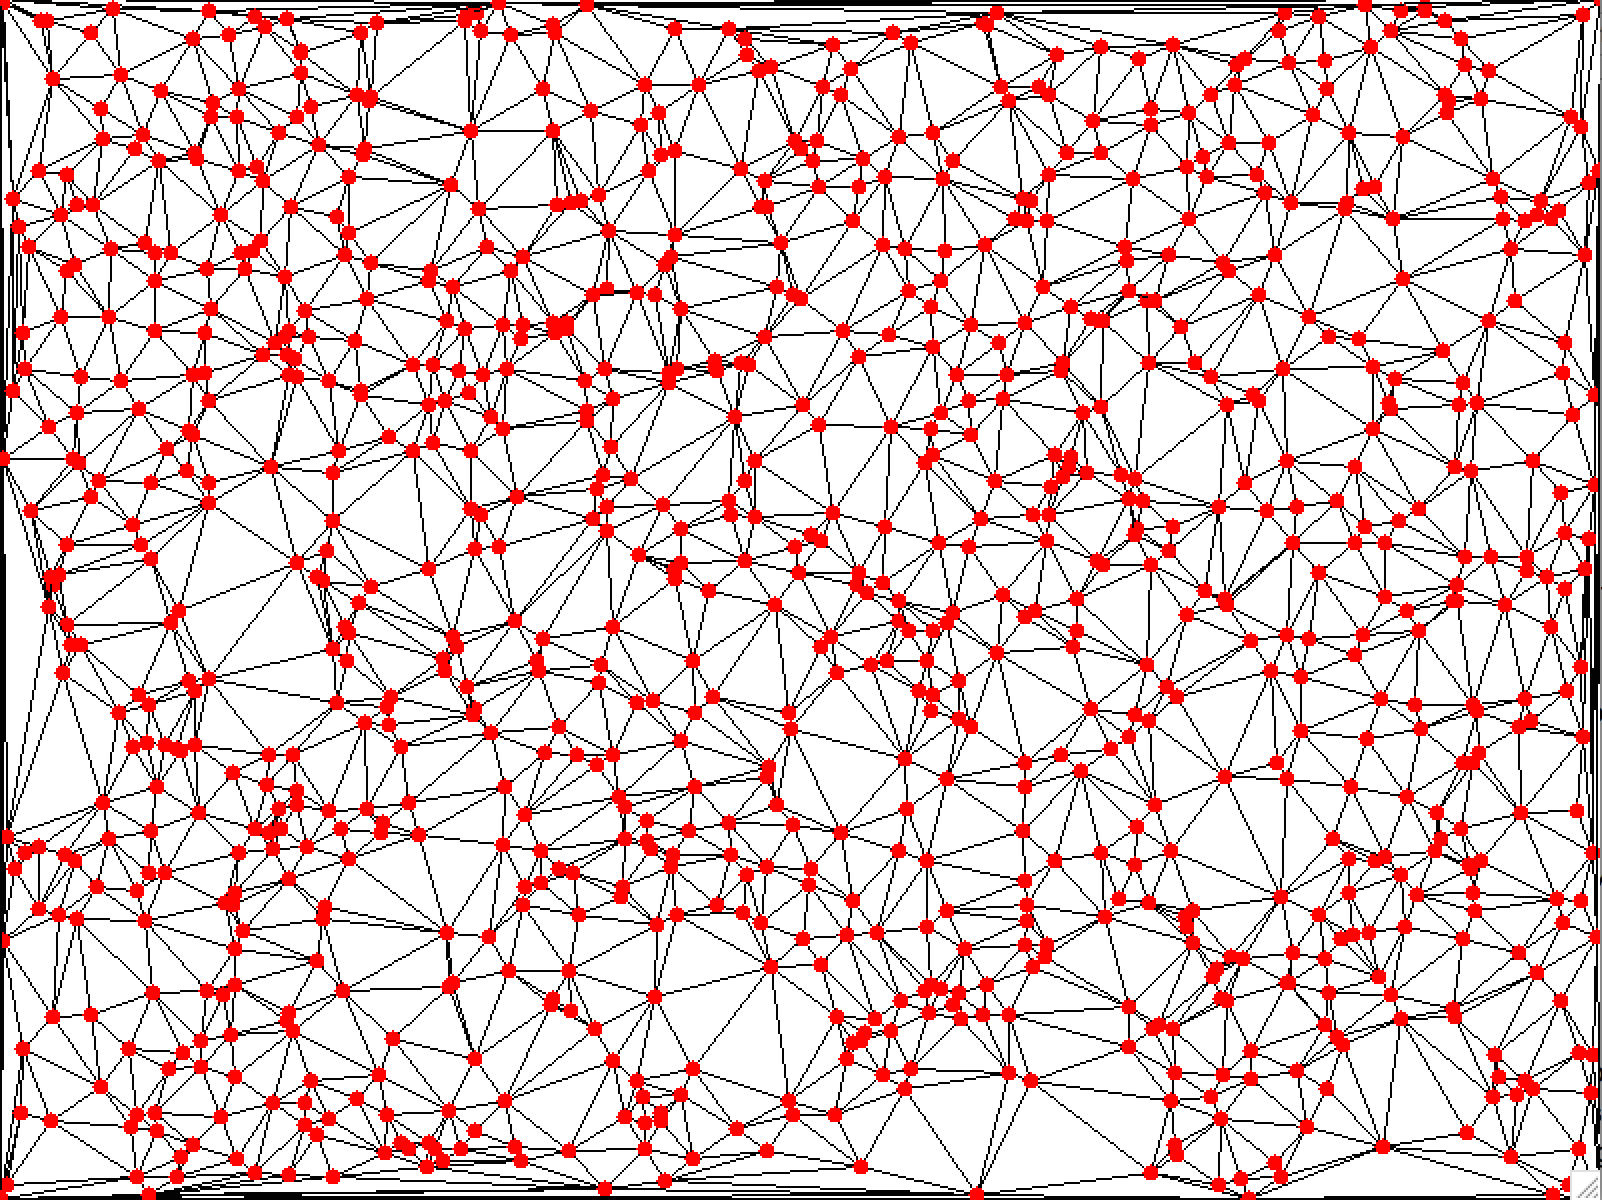
\includegraphics[height=0.5\textheight]{basic.png} \hspace*{\fill}
			\end{column}
			\begin{column}{.45\textwidth}
				\begin{itemize}
					\item Simple, easy to understand;
					\item not optimized.
				\end{itemize}
			\end{column}
		\end{columns}
	\end{frame}

	
	\section{Advanced features}
	\begin{frame}
		\frametitle{Advanced features}
		\tableofcontents[currentsection]
	\end{frame}
	
	\begin{frame}
		\frametitle{Computing the convex hull}
		Gift wrapping algorithm :
		\begin{itemize}
			\item find the lowest point ;
			\item find the next point in the convex hull to have the largest angle.
		\end{itemize}
	\end{frame}
	
	\begin{frame}
		\frametitle{Creating the first triangles}
		\begin{block}{Methods tried}
			\begin{itemize}
				\item adding a point in the center ;
				\item cut in half recursively.
			\end{itemize}
		\end{block}
	\end{frame}
	
	\begin{frame}
		\frametitle{Nearly flat triangles}
		\begin{columns}[T]
			\begin{column}{.5\textwidth}
				\hspace*{0cm} 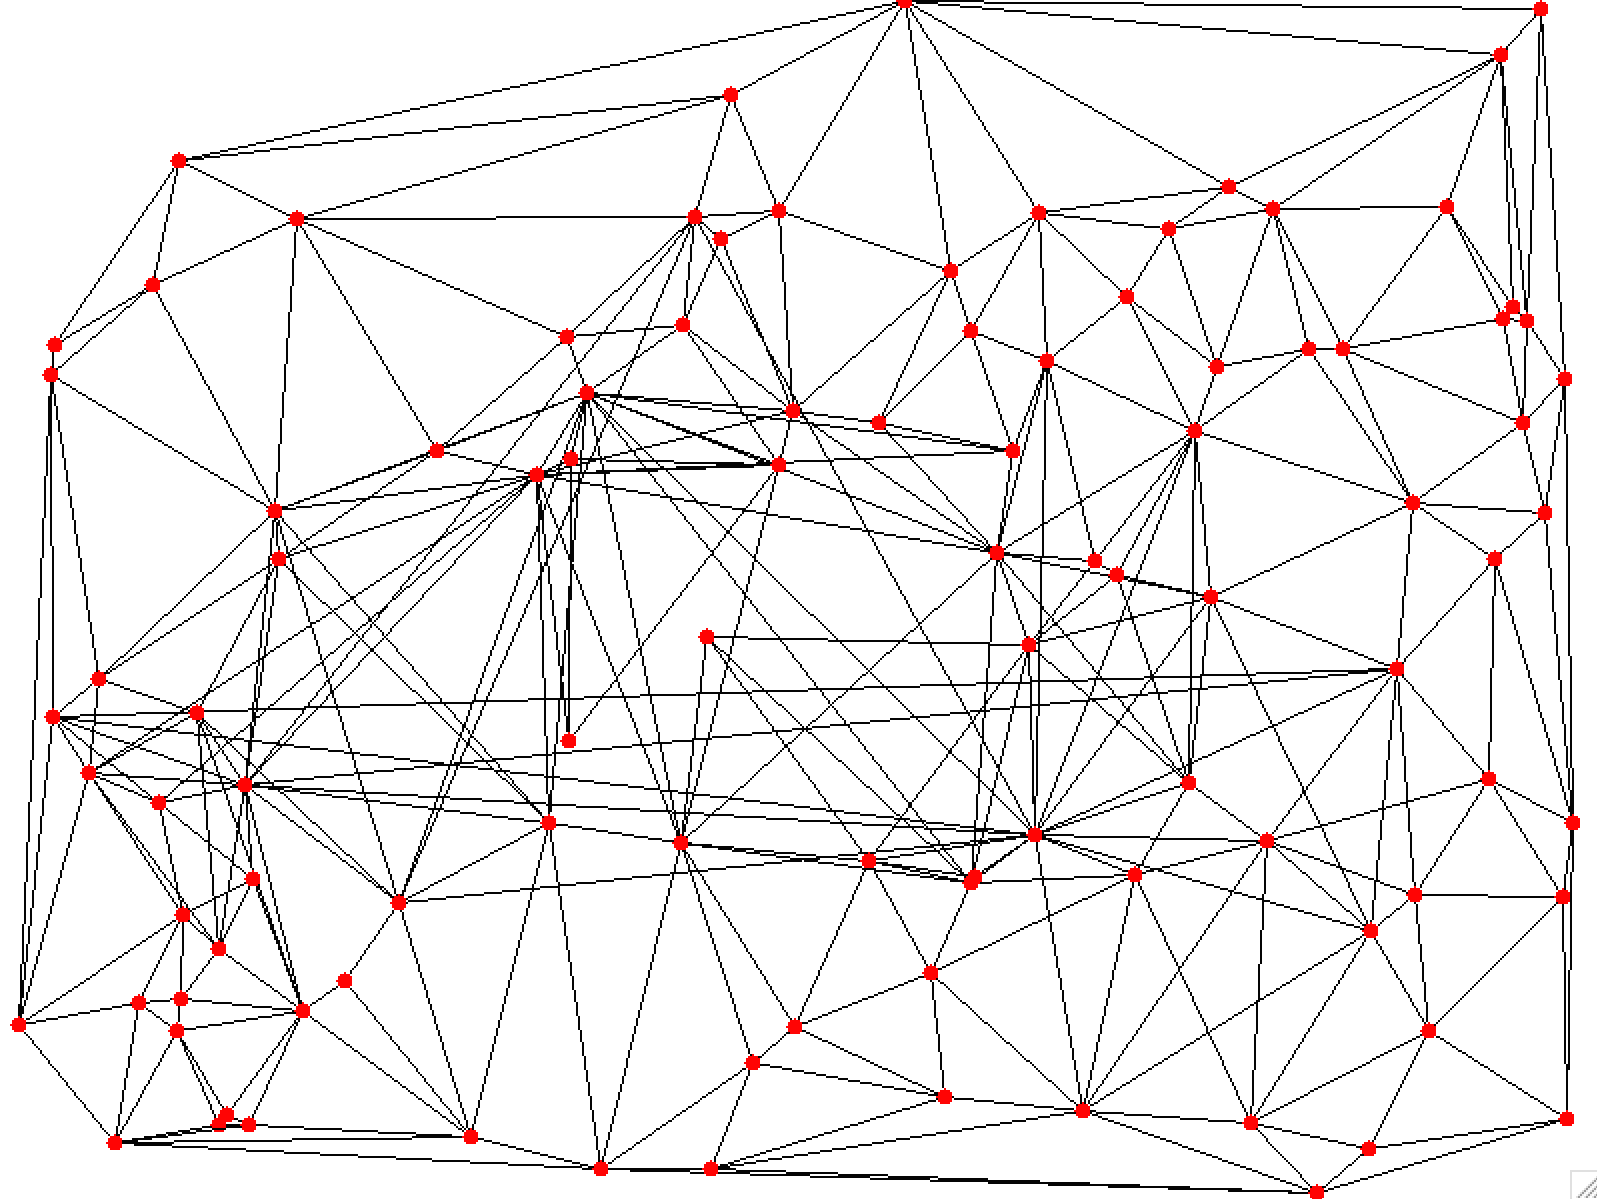
\includegraphics[height=0.5\textheight]{convexhull-messedup-abit.png} \hspace*{\fill}
			\end{column}
			\begin{column}{.45\textwidth}
				Issue with crossing edges because of huge circumscribed circles facing toward the center.
			\end{column}
		\end{columns}
	\end{frame}

	
	\section*{Conclusion}
	\begin{frame}
		\frametitle{Conclusion}
		\begin{block}{Possible improvements}
			\begin{itemize}
				\item making it work;
				\item enhance complexity.
			\end{itemize}
		\end{block}
	\end{frame}
	
	
	\begin{frame}
		\frametitle{~}
		\begin{center}
			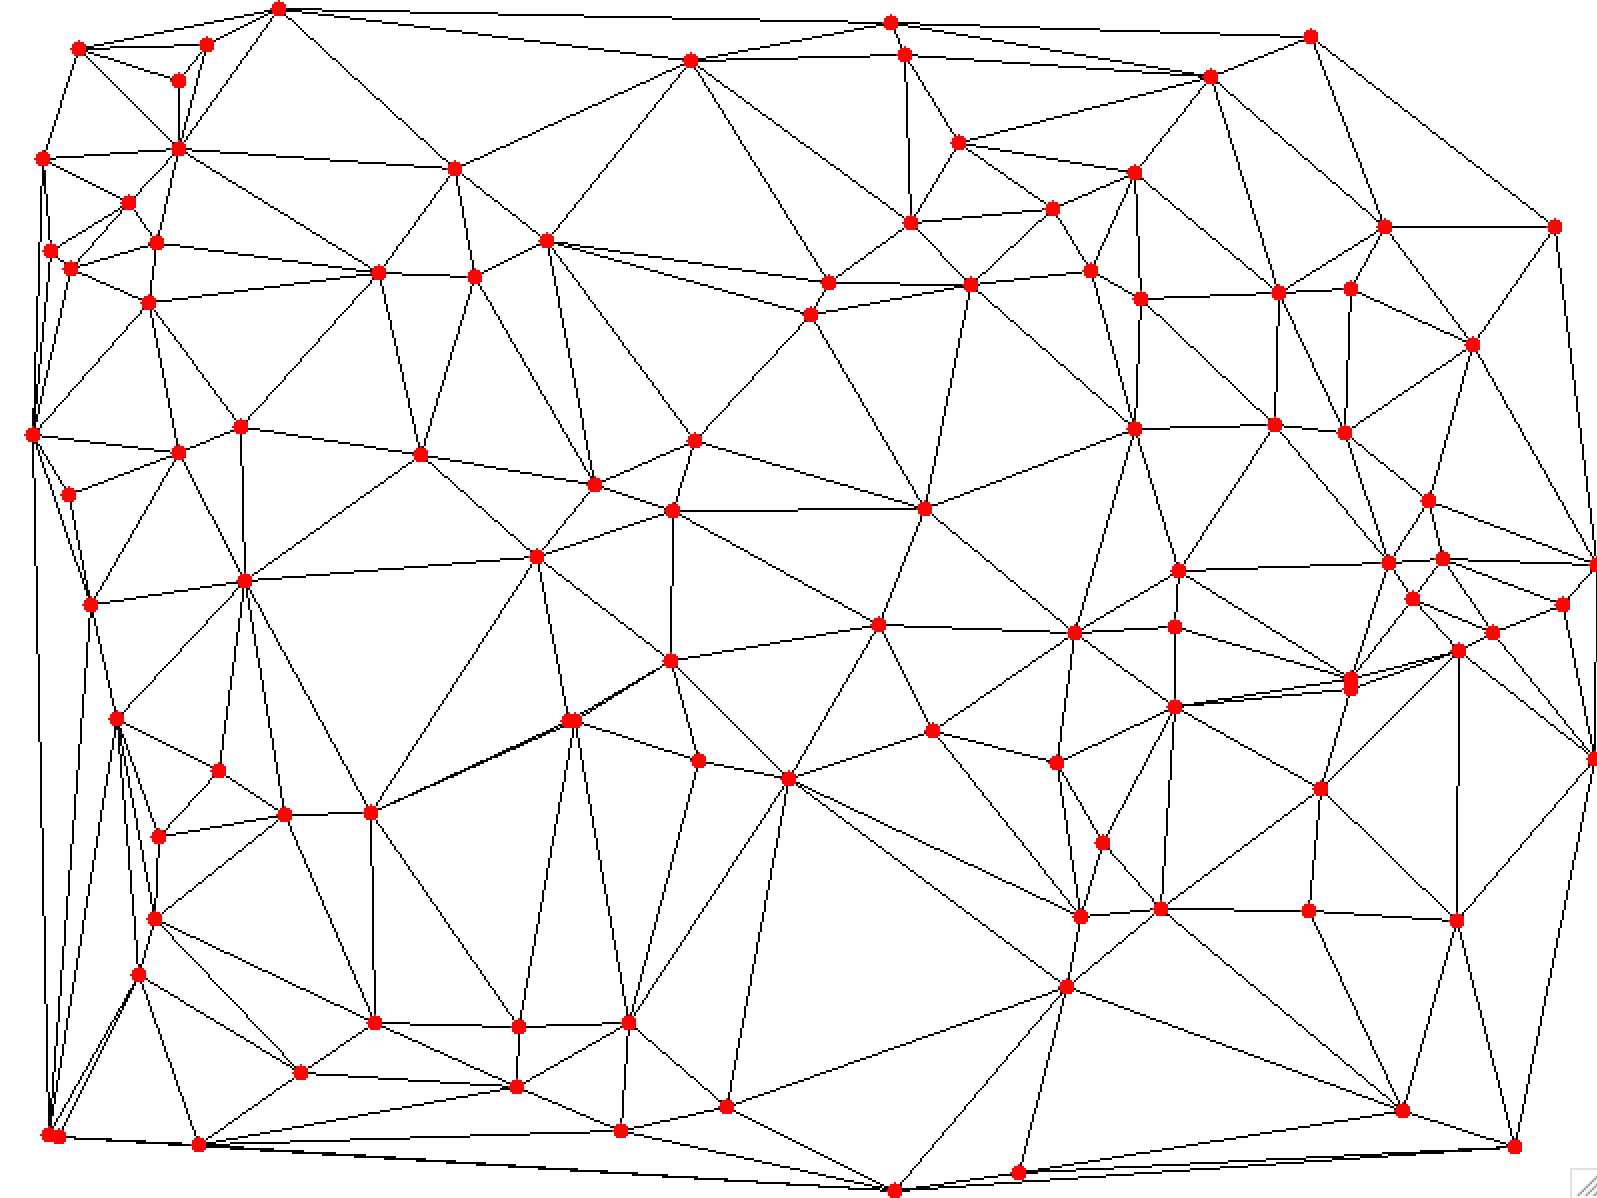
\includegraphics[scale=0.3]{convexhull-good.png}
		\end{center}
	\end{frame}

\end{document}
